\chapter{A Use Case: Training Deep Neural Network Models using Smart Scheduler}
\label{UseCase.ch}

With software frameworks like HARP, which can profile workloads (such as a family of DNN models or an animal ecology model like MegaDetector v5), build and select specific runtime estimators, and the iScheduler Framework, which invokes these estimators for user workloads, validates executions on the CI database, and monitors job scheduling. This chapter presents two key use cases. First, we demonstrate building scalable estimators using deep neural networks (DNNs), specifically convolutional neural networks (CNNs), which are widely used for image processing and pattern recognition tasks. Then, we showcase a use case in animal ecology, illustrating the interaction of iScheduler with HARP for workload management and execution.


\section{Building scalable estimators for DNN-based workloads}
\label{ScaleEstimator}

One of the key bottlenecks in the HARP framework is its dependency on manually generating training datasets. Despite adopting the scaled-down (SD) and full-scale (FS) sampling approach, workloads must still be generated for every new application. For instance, when training a new neural network model for image classification, new profiling data is required.
While analyzing estimation models built over a family of convolutional neural networks (CNNs)—referred to as a “Family of DNNs”—we found empirical evidence that models trained on data generated for certain CNN architectures (e.g., VGG16, ResNet50) can scale to other CNNs (e.g., InceptionV3).
Table~\ref{tab:CNN_Scale} presents the scalability performance of two regression models—Simple Neural Network Regressor (1LHNN) and Decision Tree Regressor (DTR)—within the Family of DNNs. Both models treat the CNN architecture as a single feature (denoted as “@model” in Figure~\ref{fig:features_overview}). 

\begin{table}[]
\caption{
Experiments demonstrate the transferability of regression models within a family of applications. }
\label{tab:CNN_Scale}
\begin{tabular}{|crrrrrrrr|}
\hline
\multicolumn{1}{|c|}{\multirow{5}{*}{\begin{tabular}[c]{@{}c@{}}Source \\ of \\ Training \\ data\\ (Below)\end{tabular}}} & \multicolumn{8}{c|}{Target Application - TA (Test Data)} \\ \cline{2-9} 
\multicolumn{1}{|c|}{} & \multicolumn{4}{c|}{VGG16} & \multicolumn{4}{c|}{InsV3} \\ \cline{2-9} 
\multicolumn{1}{|c|}{} & \multicolumn{2}{c|}{1LHNN} & \multicolumn{2}{c|}{DTR} & \multicolumn{2}{c|}{1LHNN} & \multicolumn{2}{c|}{DTR} \\ \cline{2-9} 
\multicolumn{1}{|c|}{} & MAE & \multicolumn{1}{r|}{UPP} & MAE & \multicolumn{1}{r|}{UPP} & MAE & \multicolumn{1}{r|}{UPP} & MAE & UPP \\
\multicolumn{1}{|c|}{} & MPE & \multicolumn{1}{r|}{UPAM} & MPE & \multicolumn{1}{r|}{UPAM} & MPE & \multicolumn{1}{r|}{UPAM} & MPE & UPAM \\ \hline
\multicolumn{1}{|c|}{\multirow{2}{*}{VGG16}} & \textbf{1043} & \multicolumn{1}{r|}{\textbf{10.5}} & \textbf{1272} & \multicolumn{1}{r|}{\textbf{26.31}} & 3283 & \multicolumn{1}{r|}{0.00} & 305 & 52.63 \\
\multicolumn{1}{|c|}{} & \textbf{741} & \multicolumn{1}{r|}{\textbf{1.4x}} & \textbf{369} & \multicolumn{1}{r|}{\textbf{1.3x}} & 1249 & \multicolumn{1}{r|}{1x} & 252 & 2.1x \\ \hline
\multicolumn{1}{|c|}{\multirow{2}{*}{RN50}} & 3224 & \multicolumn{1}{r|}{5.26} & 253 & \multicolumn{1}{r|}{21.05} & 1295 & \multicolumn{1}{r|}{15.78} & 1197 & 5.26 \\
\multicolumn{1}{|c|}{} & 1191 & \multicolumn{1}{r|}{2.1x} & 78 & \multicolumn{1}{r|}{2.4x} & 216 & \multicolumn{1}{r|}{3.8x} & 465 & 4.6x \\ \hline
\multicolumn{1}{|c|}{\multirow{2}{*}{InsV3}} & 51229 & \multicolumn{1}{r|}{0.00} & 426 & \multicolumn{1}{r|}{36.84} & \textbf{1041} & \multicolumn{1}{r|}{\textbf{0.00}} & \textbf{1058} & \textbf{0.00} \\
\multicolumn{1}{|c|}{} & 20378 & \multicolumn{1}{r|}{5.0x} & 179 & \multicolumn{1}{r|}{3.7x} & \textbf{603.08} & \multicolumn{1}{r|}{\textbf{1.1x}} & \textbf{545.24} & \textbf{2.4x} \\ \hline
\multicolumn{1}{|c|}{\multirow{2}{*}{**MIX}} & \textbf{139} & \multicolumn{1}{r|}{\textbf{10.52}} & 1733 & \multicolumn{1}{r|}{10.52} & 524 & \multicolumn{1}{r|}{0.00} & 1246 & 5.2 \\
\multicolumn{1}{|c|}{} & \textbf{81} & \multicolumn{1}{r|}{\textbf{1.5x}} & 509 & \multicolumn{1}{r|}{1.8x} & 123 & \multicolumn{1}{r|}{2.0x} & 808 & 1.6x \\ \hline
\multicolumn{9}{|l|}{\begin{tabular}[c]{@{}l@{}}** MIX =\textgreater usining estining training data with a few profiles from target application to \\ build estimators. Models = \{VGG16, InceptionV3, ResNet50\}, and (Models - TA) \\ refers to removing the scaled-down (SD) training data for the Target Application (TA) \\ while including only full-scale samples from TA. This setup tests the scalability of \\ estimators across different CNN architectures within the same model family.\end{tabular}} \\ \hline
\end{tabular}
\end{table}



Expanding this study, we assess how well the scalability approach extends to adapting from other neural network architectures, such as a fully connected convolutional neural network (FCNN) for image classification, while evaluating its accuracy and cost implications.



Table \ref{tab:ScaleCNN} presents the results of execution time estimation for a target application—training a VGG16 model on Wiki Images to estimate a person's age. In the first experiment, we build estimators for VGG16 using training data generated from its own emulated executions (both scaled-down (SD) and full-scale (FS) runs). Here, we run HARP end-to-end, generating SD and FS emulations, training models on this data, and building the estimators. In the second experiment, we test whether borrowing training data from existing profiles—specifically from a fully connected convolutional neural network (FCNN)—can enhance estimation accuracy. Instead of generating new scaled-down (SD) runs for VGG16, we only emulate full-scale (FS) runs, then train models on a combined dataset that includes both the newly generated FS data for VGG16 and the previously emulated FCNN data (both SD and FS samples). This approach evaluates whether leveraging existing emulated data from similar models can improve estimation performance while reducing the cost of generating new training data.


\begin{table}[]
\centering
\caption{Comparing Runtime Estimators for Predicting VGG16 Training Time: Evaluating estimators built exclusively from VGG16 emulations versus those incorporating VGG16 data into existing CNN-based emulations.}
\label{tab:ScaleCNN}
\begin{tabular}{|c|crr|c|c|}
\hline
\multirow{3}{*}{\textbf{\begin{tabular}[c]{@{}c@{}}Prediction\\ Model\end{tabular}}} & \multicolumn{3}{c|}{\multirow{2}{*}{\textbf{\begin{tabular}[c]{@{}c@{}}Walltime Error \\ (Actual, Predicted)\end{tabular}}}} & \multirow{3}{*}{\textbf{\begin{tabular}[c]{@{}c@{}}Training \\ Samples\end{tabular}}} & \multirow{3}{*}{\textbf{\begin{tabular}[c]{@{}c@{}}New Data \\ Generation\\ Cost (in \$)\end{tabular}}} \\
 & \multicolumn{3}{c|}{} &  &  \\ \cline{2-4}
 & \multicolumn{1}{c|}{\textbf{MAE}} & \multicolumn{1}{c|}{\textbf{MAPE}} & \multicolumn{1}{c|}{\textbf{UPP}} &  &  \\ \hline
\multicolumn{1}{|l|}{\textbf{VGG16}} & \multicolumn{1}{r|}{1043} & \multicolumn{1}{r|}{701} & 11 & \multicolumn{1}{r|}{511} & \multicolumn{1}{r|}{5.15} \\ \hline
\multicolumn{1}{|l|}{\textbf{Fully-CNN}} & \multicolumn{1}{r|}{\textbf{116}} & \multicolumn{1}{r|}{\textbf{56}} & \textbf{0} & \multicolumn{1}{r|}{\textbf{775}} & \multicolumn{1}{r|}{\textbf{1.35}} \\ \hline
\end{tabular}
\end{table}

By leveraging an existing dataset, we learn execution behaviors from similar models and reduce data generation costs from \$5.15 to \$1.35. The availability of multiple training emulations for similar models improves prediction accuracy across MAE (Mean Absolute Error), MAPE (Mean Absolute Percentage Error), and UPP (Under-Prediction Percentage) while minimizing the need for additional application-specific emulations.



\section{iScheduler Workflow for DNN and MegaDetector Training Job Executions}


\begin{figure}[]
    \centering    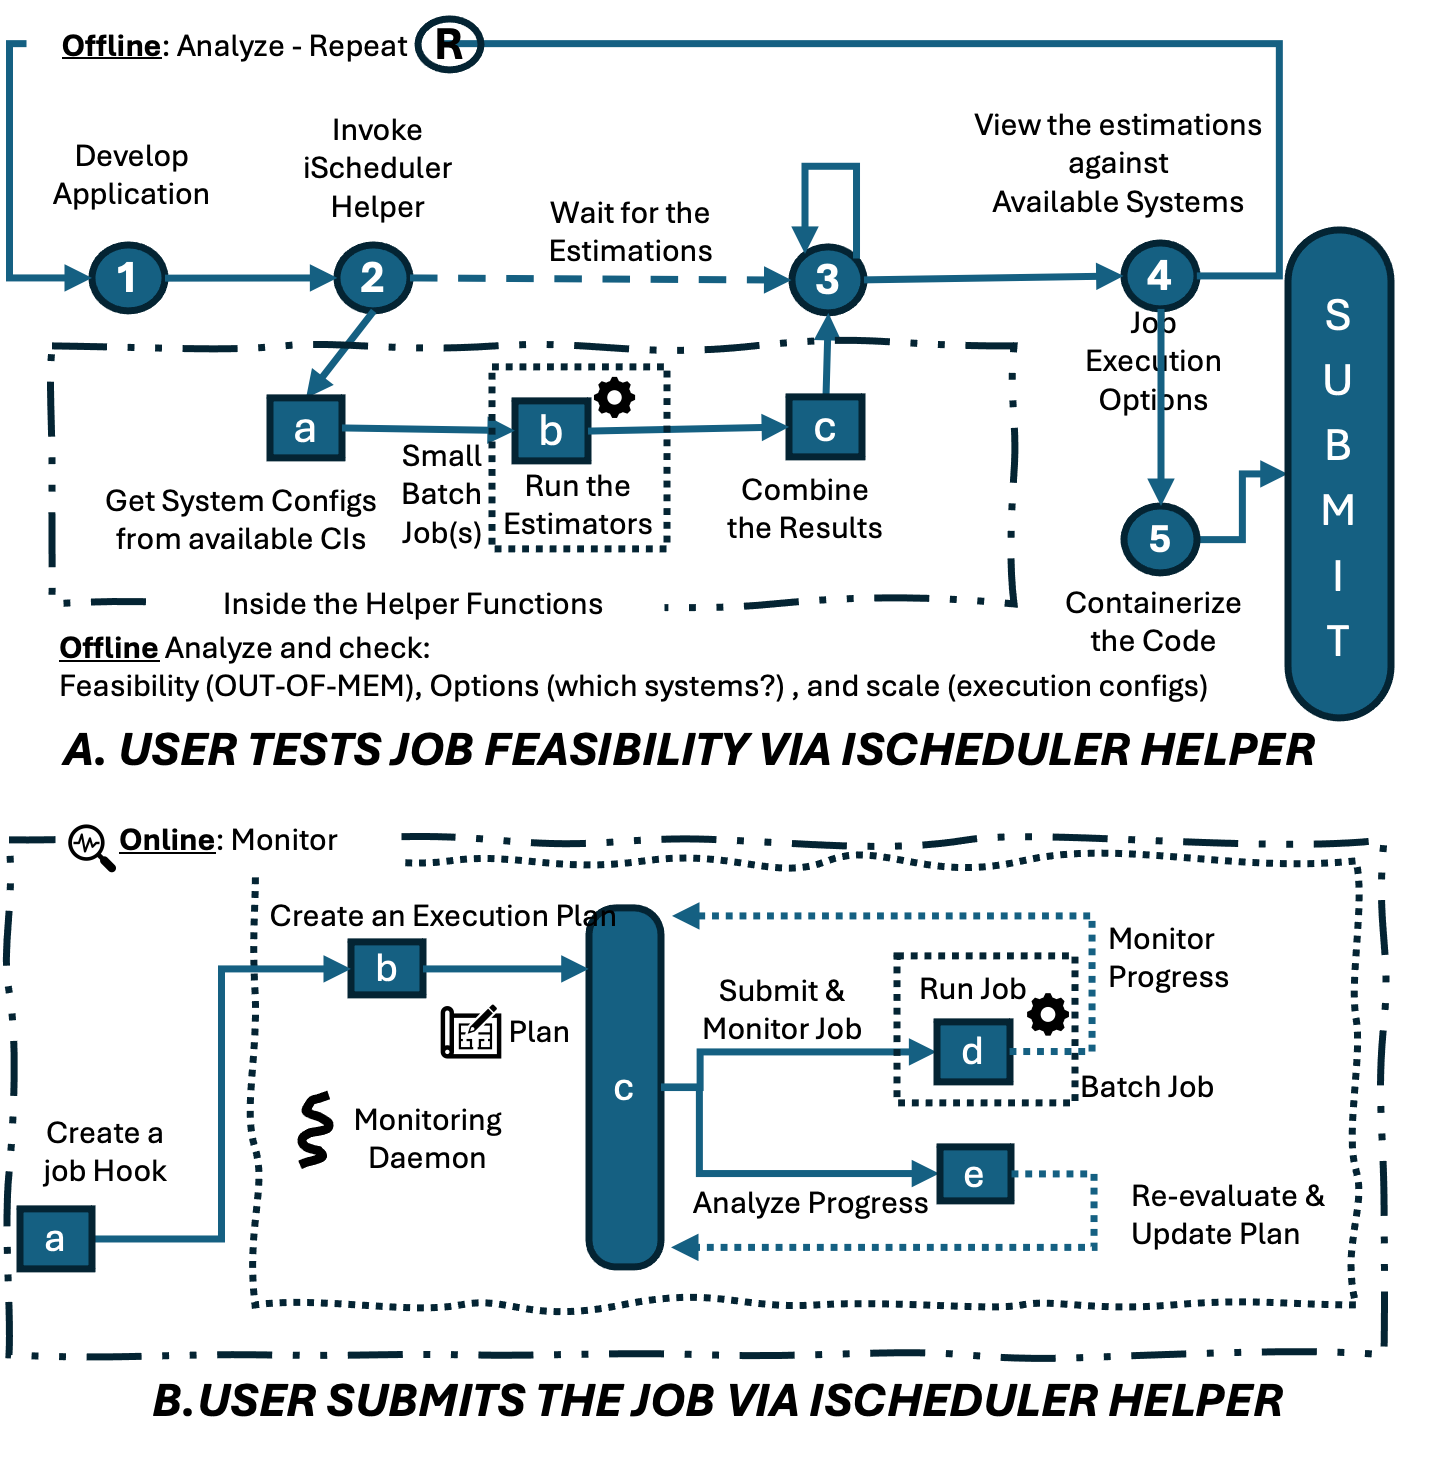
\includegraphics[width=\textwidth]{Images/ISchedulerPipeline.png}
    \caption{Workflow of the iScheduler framework, illustrating both offline analysis and online monitoring phases. The process consists of multiple steps, including workload profiling, resource validation, job submission, and monitoring.}
    \label{fig:iSchedulerPipeline}
\end{figure}

Figure \ref{fig:iScheduler} outlines the components of the \textbf{iScheduler framework}, while Figure \ref{fig:iSchedulerPipeline} illustrates user interaction with the framework through the \textbf{iScheduler Helper module}. This module allows users to assess their \textbf{job's resource requirements} against available systems, facilitating \textbf{job execution orchestration} with the \textbf{Intelligence Plane}.  

In this section, we walk through two use cases:  
\begin{enumerate}
    \item \textbf{Training a ResNet50 model using the scheduled framework}, leveraging previously trained models (as discussed in \textbf{Section \ref{ScaleEstimator}}) to provide \textbf{feasibility options} and execute the training job.  
    \item \textbf{Using an iScheduler framework notebook endpoint} to \textbf{validate feasibility and execute training jobs} for \textbf{animal ecology model training with MegaDetector}.  
\end{enumerate}

\subsection{Use Case 1: Training a ResNet50}
\label{usecase_trainresnet}
A user aims to train a ResNet50 vision model with 20k images over 50 epochs, optimizing accuracy by testing different batch sizes. They interact with the iScheduler Helper to assess runtime requirements and batch-scaling feasibility across available CI systems. The workloads are executed as single-node allocations managed through TAPIS, with in-application checkpointing and callbacks ensuring job continuity and monitoring progress.

\textbf{Workflow:} The interaction between the user and the Smart Scheduler follows these steps:
\begin{itemize}
    \item After configuring the ResNet50 architecture, the user invokes the appropriate iScheduler Helper function, providing model details and target batch sizes (32, 64).
    \item The Helper Function retrieves node configurations (CPU and GPU node specs for Pitzer Cluster) from the CI database and runs estimators to provide resource predictions.
    \item The user reviews the estimations and selects an execution plan, either manually submitting the job or delegating it to the Intelligence Plane. 
    \item \textbf{Resource Estimation Results:}
    \begin{itemize}
        \item \textbf{Pitzer CPU Node:} Can execute ResNet50 for both batch sizes with estimated execution times of 9.2 hours (batch size 32) and 9.7 hours (batch size 64), with corresponding costs of \$0.7728 and \$0.7308, respectively.
        \item \textbf{Pitzer GPU Node (32 GB Memory):} Can handle only batch size 32, with an estimated execution time of 2.4 hours and a cost of \$0.4176.
    \end{itemize}
    \item The user has two options after reviewing estimation results:
    \begin{itemize}
        \item Manual Submission: Configure a SLURM script to submit the job independently.
        \item Delegated Execution: Allow the Intelligence Plane to handle job submission and monitoring.
    \end{itemize}
    \item The prototype demonstrates two execution feasibilities:
    \begin{itemize}
        \item Ideal System Configurations: Submitting with the best possible configurations to minimize interruptions.
        \item Availability-Based Execution: Adapting to CI queue states, such as number of idle nodes and pending jobs.
    \end{itemize}
    \item The user containerizes the code, publishes it to a publicly accessible location, and creates a TAPIS Application.
    \item The Intelligence Plane manages job execution, submission, and progress monitoring via callbacks. Jobs exceeding the maximum walltime are handled as cascading tasks, with reassessments and AI-driven finetuning loops optimizing memory and walltime estimations.
    \item \textbf{Execution Strategy Comparison:}
    \begin{itemize}
        \item \textbf{Ideal Configuration (Pitzer GPU):} Estimated job completion 28 hours (26 hours wait time + 2 hours execution) with a cost of \$0.348.
        \item \textbf{Availability-Based Execution:} Estimated job completion 9 hours (immediate resource allocation) with a cost of \$0.756.
    \end{itemize}
\end{itemize}

Given the GPU node wait time, the current ResNet50 training job could be completed on a CPU node before the GPU allocation becomes available, potentially saving researchers valuable time.



\subsection{Use Case 2: Training a MegaDetectorV5}
\label{uesecase_trainmegadetector}
The primary objective of this use case is to leverage the iScheduler Framework integrated with TAPIS to help ecologists efficiently fine-tune their models.

\subsubsection{Adapting MegaDetector for Small Animal Ecosystem Monitoring}

Ecologists study small animal ecosystems by collecting data using the Adapted Hunt Drift Fence Technique (AHDriFT), which enhances detection by guiding small animals into a bucket equipped with a camera trap \cite{CITE}. Conducted by the Ohio Department of Natural Resources, this survey generated a benchmark dataset of 120,000 annotated images, covering 7 order-level and 45 species-level categories, including small mammals, reptiles, and amphibians commonly found in Ohio.  

The camera trap edge device deployed in the field consists of a motion sensor, a camera, and a small computing unit (e.g., a Raspberry Pi) to run inference models. When the sensor detects movement, it triggers the camera to capture a burst of images to record the object that activated the motion detection. These images are then analyzed by an inference model, such as MegaDetector \cite{CITE}, running on the edge device to classify the object as either an animal or non-animal motion (e.g., leaf movement). Only relevant images are stored, significantly conserving storage space, as approximately 70\% of captured images on camera traps are empty frames, which would otherwise quickly fill the device’s limited storage.  

\subsubsection{Challenges in Deploying Pretrained MegaDetector Models}

Deploying an off-the-shelf pretrained MegaDetector model on the edge device proved inefficient due to mismatches in training data. Existing MegaDetector models were primarily trained on larger animals, whereas the Ohio Small Animal Survey dataset includes small rodents, insects, and other tiny species. The survey utilizes ground-facing cameras with a consistent background, minimizing noise and false triggers. In contrast, MegaDetector’s pretrained models were trained on side-facing camera traps, capturing highly varied environmental backgrounds, leading to greater variation in lighting conditions, occlusions, and motion artifacts.  

Due to these substantial differences, researchers need to fine-tune the MegaDetector model on this representative dataset before deployment on the edge device. Fine-tuning ensures the model effectively identifies small animals while filtering out irrelevant detections.  

\subsubsection{Interactive Training \& Scheduling with iScheduler}

Researchers can interact with the iScheduler Notebook Interface \cite{LINK} to assess the cost and feasibility of fine-tuning MegaDetector and execute training jobs using the scheduler interface. The iScheduler Notebook or TAPIS can be used to monitor training progress, whether as a single job or a series of sequential jobs scheduled based on resource availability. This dynamic scheduling approach ensures efficient resource allocation for fine-tuning, improving model adaptability for small-animal detection in edge environments.

\begin{figure}[]
    \centering
    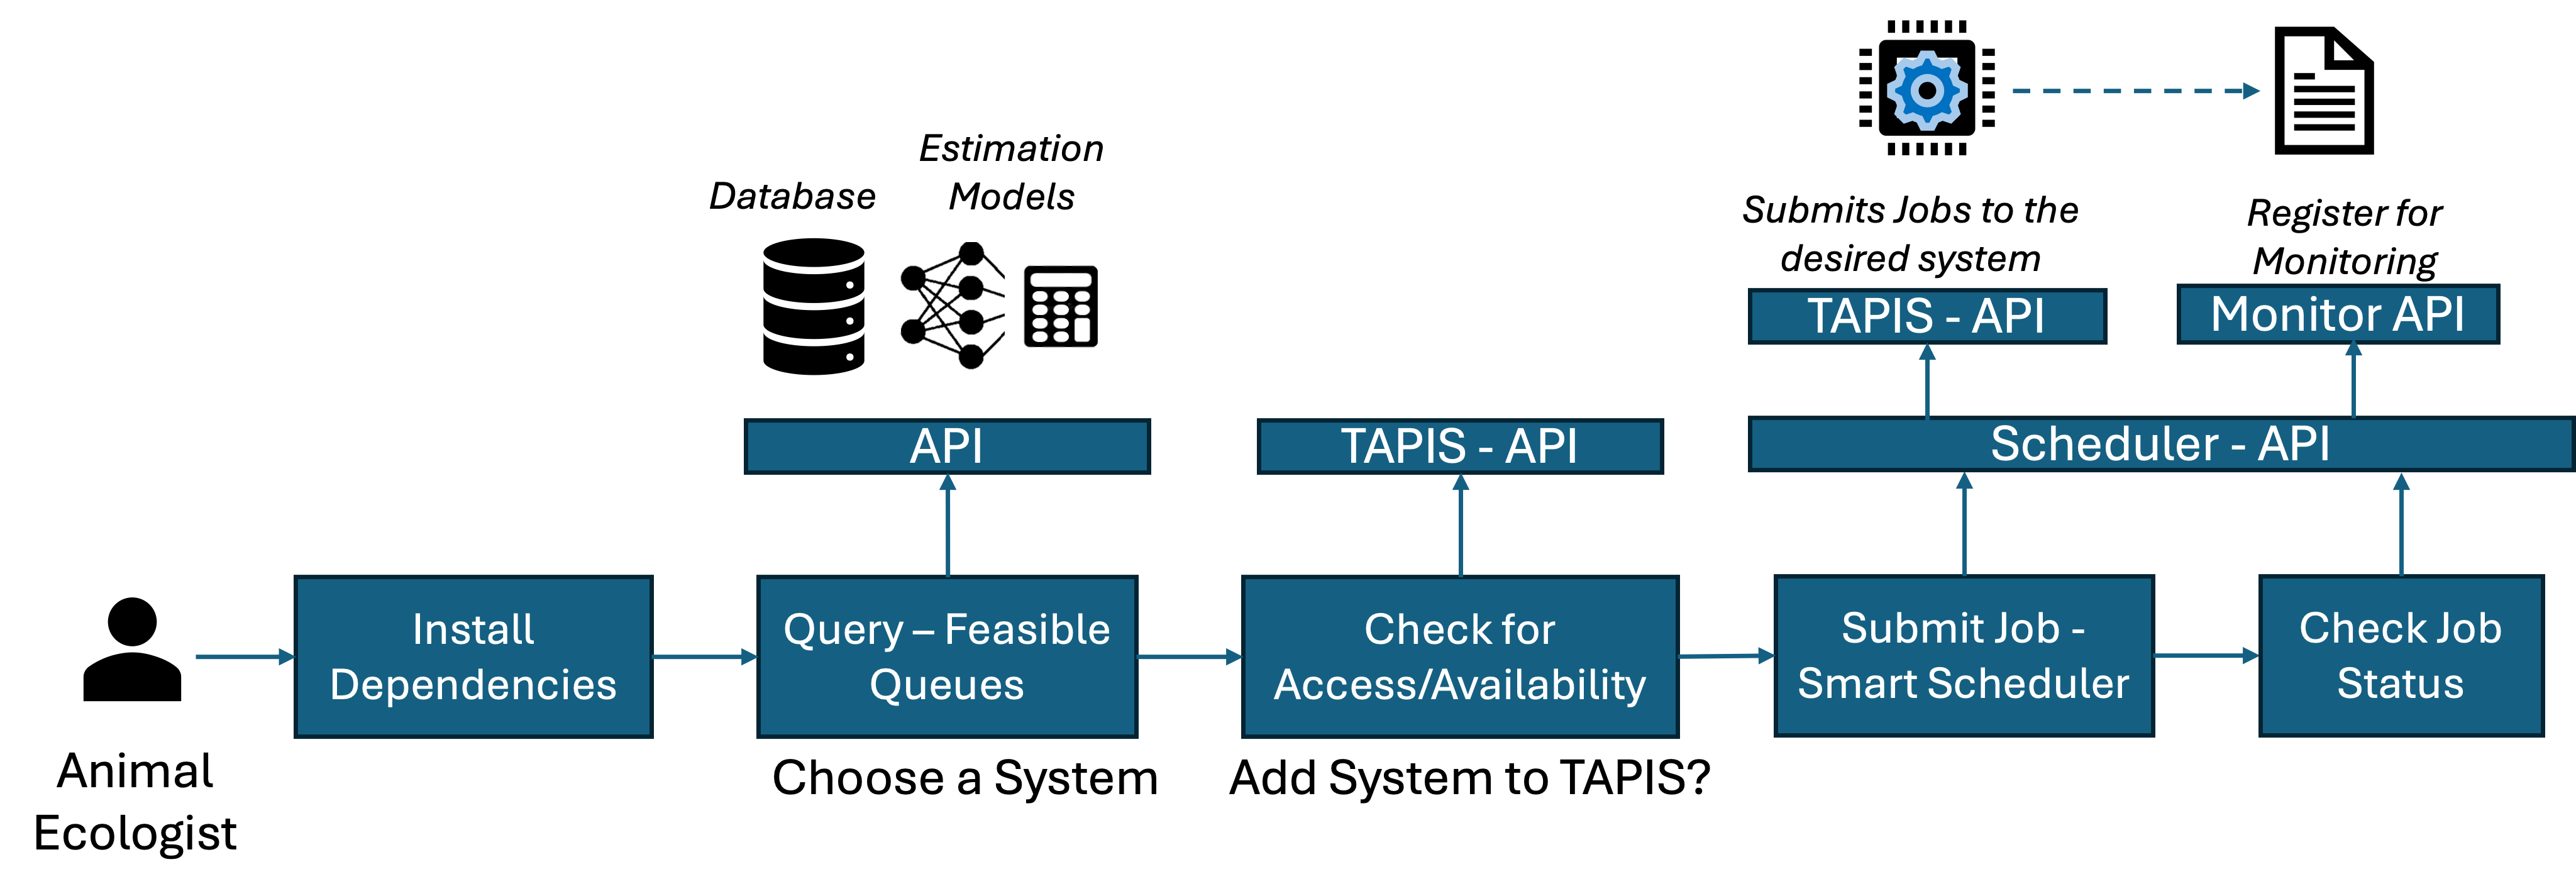
\includegraphics[width=\textwidth]{Images/TAPIS_AE1.png}
    \caption{Workflow illustrating the steps an ecologist follows when interacting with the iScheduler Framework. The process includes installing dependencies, querying feasible queues, checking access, submitting jobs, and monitoring execution status through TAPIS and Scheduler APIs.}
    \label{fig:iScheduler_TAPIS_Workflow}
\end{figure}

Figure \ref{fig:iScheduler_TAPIS_Workflow} illustrates the steps an ecologist follows while interacting with the \textbf{iScheduler Framework}:

\begin{enumerate}
    \item \textbf{Install Dependencies:}  
    Download and install the necessary components, including the Smart Scheduler and MegaDetector dependencies, from GitHub.  
   
    \item \textbf{Query Feasible Queues:}  
    Interact with the iScheduler Database Helper functions via the API to determine feasible execution queues for available systems registered in TAPIS (including all OSC and TACC resources).  Table \ref{tab:AE_cost} shows a snapshot into the estion feasibility results. 

    \item \textbf{Check for Access and Availability:}  
    Verify access permissions for the identified systems. If a system offers a better cost-turnaround time, users may request access to TACC or OSC.  

    \item \textbf{Submit Jobs via Smart Scheduler:}  
    Submit the job using the Smart Scheduler API, which handles execution on the selected system.  

    \item \textbf{Monitor Job Status:}  
    Track job execution through the Scheduler API or directly via TAPIS Monitor API.  
\end{enumerate}

\begin{table}[]
\caption{Cost estimation for fine-tuning the MegaDetector model based on fine-tuning predictions across different queues.}
\label{tab:AE_cost}
\begin{tabular}{|l|l|r|r|c|r|}
\hline
cluster\_name & queue\_name & \begin{tabular}[c]{@{}r@{}}MaxMemory\\ (MB)\end{tabular} & \begin{tabular}[c]{@{}r@{}}Max\\ Minutes\end{tabular} & \multicolumn{1}{l|}{Feasible} & \begin{tabular}[c]{@{}r@{}}Computed\\ \_Cost (\$)\end{tabular} \\ \hline
owens & \begin{tabular}[c]{@{}l@{}}condo-PYS1124-\\ backfill-serial\end{tabular} & 120820 & 360 & No & 0.000 \\
owens & \begin{tabular}[c]{@{}l@{}}gpubackfill-\\ parallel\end{tabular} & 120820 & 240 & Yes & 22.320 \\
owens & debug & 120820 & 60 & No & 0.000 \\
pitzer & \begin{tabular}[c]{@{}l@{}}condo-osumed-gpu-\\ 48core-backfill-serial\end{tabular} & 371712 & 240 & Yes & 22.320 \\
pitzer & CPU-serial & 182240 & 360 & Yes & 1.080 \\
pitzer & \begin{tabular}[c]{@{}l@{}}condo-gao-gpu-\\ backfill-serial\end{tabular} & 371712 & 60 & No & 0.000 \\
pitzer & \begin{tabular}[c]{@{}l@{}}condo-osumed-gpu-\\ 48core-backfill-parallel\end{tabular} & 371712 & 240 & Yes & 22.320 \\ \hline
\end{tabular}
\end{table}